% ------------------------------------------------------------------------------
% TYPO3 CMS 7.1 - What's New - Chapter "Introduction" (Dutch Version)
%
% @author	Michael Schams <schams.net>
% @license	Creative Commons BY-NC-SA 3.0
% @link		http://typo3.org/download/release-notes/whats-new/
% @language	Dutch
% ------------------------------------------------------------------------------
% LTXE-CHAPTER-UID:		947f71fe-f93742b1-4879d61a-4a9bbcd6
% LTXE-CHAPTER-NAME:	Introduction
% ------------------------------------------------------------------------------

\section{Inleiding}
\begin{frame}[fragile]
	\frametitle{Inleiding}

	\begin{center}\huge{Inleiding}\end{center}
	\begin{center}\huge{\color{typo3darkgrey}\textbf{De feiten}}\end{center}

\end{frame}

% ------------------------------------------------------------------------------
% LTXE-SLIDE-START
% LTXE-SLIDE-UID:		c9deba87-2648f0da-8725e225-aa3d2011
% LTXE-SLIDE-ORIGIN:	a86a13ef-338d870a-beaf8e5a-65cd0eab English
% LTXE-SLIDE-TITLE:		TYPO3 CMS 7.1 - De feiten
% ------------------------------------------------------------------------------

\begin{frame}[fragile]
	\frametitle{Inleiding}
	\framesubtitle{TYPO3 CMS 7.1 - De feiten}

	\begin{itemize}
		\item Releasedatum: 24 Februari 2015
		\item Releasetype: "Sprint Release"
		\item Visie: Omarm, Innoveer, Lever
		\item Primaire focus: Opruimen en stroomlijnen van de core
	\end{itemize}

	\begin{figure}
		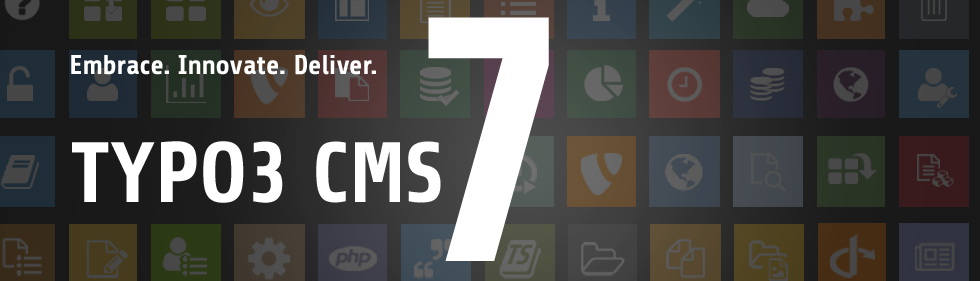
\includegraphics[width=0.95\linewidth]{typo3-seven-zero-banner.png}
	\end{figure}

\end{frame}

% ------------------------------------------------------------------------------
% LTXE-SLIDE-START
% LTXE-SLIDE-UID:		577ffee3-109687c8-99896193-3f307946
% LTXE-SLIDE-ORIGIN:	37e4488f-040dd53e-fac4a3a3-c587b0d9 English
% LTXE-SLIDE-TITLE:		System Requirements
% ------------------------------------------------------------------------------

\begin{frame}[fragile]
	\frametitle{Inleiding}
	\framesubtitle{Systeemvereisten}

	\begin{itemize}
		\item PHP*:\tabto{2.2cm}v5.5.0 - v5.6.x
		\item MySQL:\tabto{2.2cm}v5.5.x - v5.6.x (no strict mode)
		\item Schijfruimte:\tabto{2.2cm}min 200 MB
		\item PHP instellingen:

			\begin{itemize}
				\item memory\_limit >= 128M
				\item max\_execution\_time >= 240s
				\item compilatie-optie \texttt{--disable-ipv6} moet \underline{niet} worden gebruikt
			\end{itemize}

		\item Backend vereist IE >= 9 of elke andere moderne browser

	\end{itemize}

	\vspace{1cm}
	*) Meer details: \href{http://typo3.org/news/article/php-minimum-requirements-for-typo3-cms-7/}{PHP Minimum Requirements for TYPO3 CMS 7}

\end{frame}

% ------------------------------------------------------------------------------
% LTXE-SLIDE-START
% LTXE-SLIDE-UID:		1a48f591-2e8c6214-f7c329f7-20c70cc9
% LTXE-SLIDE-ORIGIN:	249e8dc9-e935b8a6-999d6e0b-c66c33b6 English
% LTXE-SLIDE-TITLE:		Development And Release Timeline
% ------------------------------------------------------------------------------

\begin{frame}[fragile]
	\frametitle{Inleiding}
	\framesubtitle{Ontwikkel en releasetraject}

	\begin{figure}
		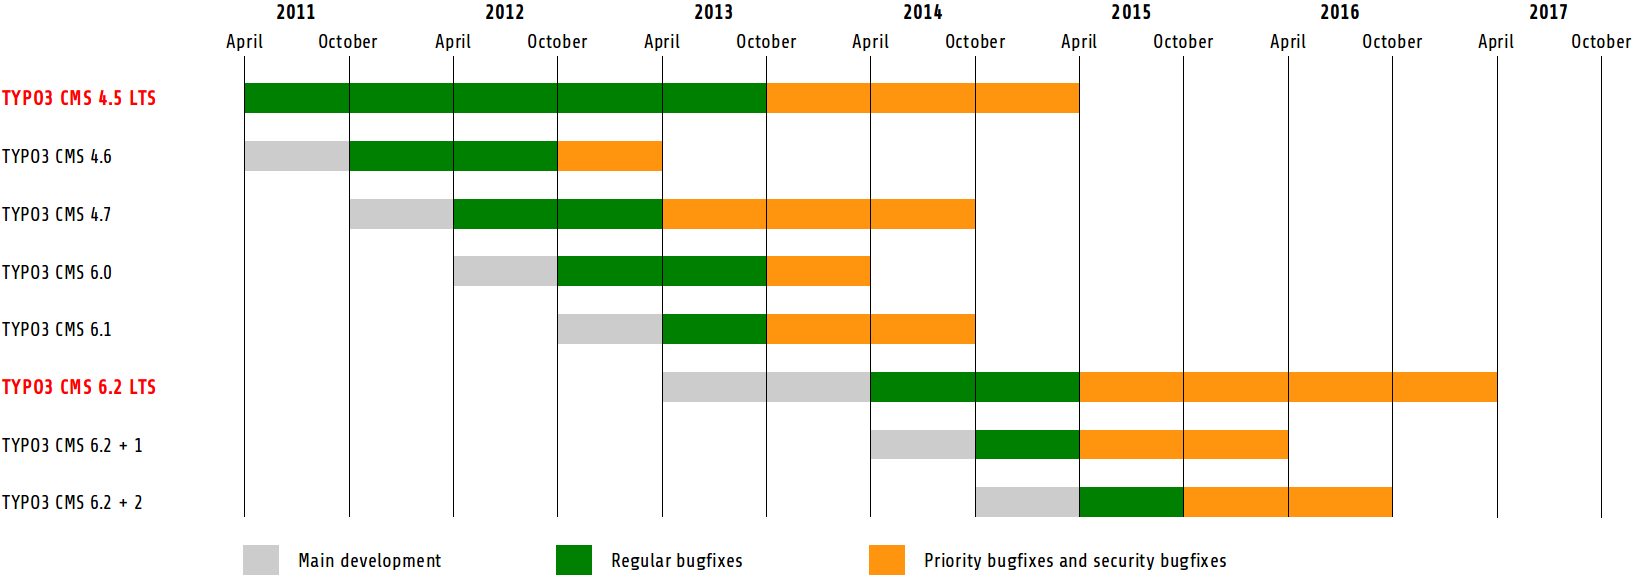
\includegraphics[width=0.90\linewidth]{Introduction/ReleaseAgenda.png}
	\end{figure}

\end{frame}

% ------------------------------------------------------------------------------
% LTXE-SLIDE-START
% LTXE-SLIDE-UID:		ff39f314-1bee8217-b3b94e66-37c6fa0b
% LTXE-SLIDE-ORIGIN:	855168a2-d07a3cc8-65f8f9bd-827ef9e9 English
% LTXE-SLIDE-TITLE:		TYPO3 CMS Roadmap
% ------------------------------------------------------------------------------
% https://typo3.org/typo3-cms/roadmap/

\begin{frame}[fragile]
	\frametitle{Inleiding}
	\framesubtitle{TYPO3 CMS Roadmap}

	Geschatte releasedatums met primaire focus:

	\begin{itemize}
		\item v7.0 \textrightarrow\tabto{1.3cm}2 dec 2014\tabto{3.4cm}Backendrevisie Deel 1

		\item
			\begingroup
				\color{typo3orange}
					v7.1 \textrightarrow\tabto{1.3cm}17/feb/2015\tabto{3.4cm}Core opschonen \& stroomlijnen
			\endgroup

		\item v7.2 \textrightarrow\tabto{1.3cm}10/maa/2015\tabto{3.4cm}Frontend
		\item v7.3 \textrightarrow\tabto{1.3cm}21/apr/2015\tabto{3.4cm}Composer Ecosysteem
		\item v7.4 \textrightarrow\tabto{1.3cm}9/jun/2015\tabto{3.4cm}Backendrevisie Deel 2
		\item v7.5 \textrightarrow\tabto{1.3cm}28/jul/2015\tabto{3.4cm}\textit{(nader te bepalen...)}
		\item v7.6 \textrightarrow\tabto{1.3cm}13/okt/2015\tabto{3.4cm}pre-LTS inferno
		\item v7.7 \textrightarrow\tabto{1.3cm}eind 2015\tabto{3.4cm}\textbf{TYPO3 CMS 7 LTS} (Long Term Release)
	\end{itemize}

	\smaller
		\url{https://typo3.org/typo3-cms/roadmap/}\newline
		\url{http://typo3.org/news/article/embrace-and-innovate-typo3-cms-7/}
	\normalsize

\end{frame}

% ------------------------------------------------------------------------------
% LTXE-SLIDE-START
% LTXE-SLIDE-UID:		b7a108de-07207c23-80da4ee3-3c49363a
% LTXE-SLIDE-ORIGIN:	0a54fbe0-06a2837d-605a5eed-6aa40506 English
% LTXE-SLIDE-TITLE:		Installation
% LTXE-SLIDE-REFERENCE:	https://forge.typo3.org/issues/62578
% ------------------------------------------------------------------------------

\begin{frame}[fragile]
	\frametitle{Inleiding}
	\framesubtitle{Installatie}

	\begin{itemize}
		\item Officiële installatieprocedure voor Linux/Mac OS X\newline
			(DocumentRoot bijvoorbeeld \texttt{/var/www/site/htdocs}):
		\begin{lstlisting}
			$ cd /var/www/site
			$ wget --content-disposition get.typo3.org/7.1
			$ tar xzf typo3_src-7.1.0.tar.gz
			$ cd htdocs
			$ ln -s ../typo3_src-7.1.0 typo3_src
			$ ln -s typo3_src/index.php
			$ ln -s typo3_src/typo3
			$ touch FIRST_INSTALL
		\end{lstlisting}

		\item Symbolische koppelingen in Microsoft Windows:

			\begin{itemize}
				\item Gebruik \texttt{junction} in Windows XP/2000
				\item Gebruik \texttt{mlink} in Windows Vista and Windows 7
			\end{itemize}

	\end{itemize}
\end{frame}

% ------------------------------------------------------------------------------
% LTXE-SLIDE-START
% LTXE-SLIDE-UID:		1b732585-da909150-11d6c403-9996817f
% LTXE-SLIDE-ORIGIN:	914dda49-a07eaf35-b9d24c58-6890a673 English
% LTXE-SLIDE-TITLE:		Upgrade to TYPO3 CMS 7
% LTXE-SLIDE-REFERENCE:	https://forge.typo3.org/issues/62578
% ------------------------------------------------------------------------------

\begin{frame}[fragile]
	\frametitle{Inleiding}
	\framesubtitle{Upgrade naar TYPO3 CMS 7.x}

	\begin{itemize}
		\item Upgrades alleen mogelijk vanaf TYPO3 CMS 6.2 LTS
		\item Oudere versies moeten eerst geüpgrade worden naar TYPO3 CMS 6.2 LTS
	\end{itemize}

	\begin{itemize}

		\item Upgrade-instructies (Engels):\newline
			\smaller\url{http://wiki.typo3.org/Upgrade#Upgrading_to_7.1}\normalsize
		\item Officiële TYPO3-handleiding (Engels) "TYPO3 Installation and Upgrading":
			\smaller\url{http://docs.typo3.org/typo3cms/InstallationGuide}\normalsize
		\item Algemene benadering:
			\begin{itemize}
				\item Controleer minimale systeemeisen \small(PHP, MySQL, etc.)
				\item Inspecteer \textbf{deprecation\_*.log} in oude TYPO3 instantie
				\item Werk alle extensies bij naar de meest recente versie
				\item Zet de nieuwe bronbestanden klaar en start de Installatie Werkset \textrightarrow Upgrade Wizard
				\item Controleer startup-module voor backend gebruikers (optioneel)
			\end{itemize}
	\end{itemize}

\end{frame}

% ------------------------------------------------------------------------------
